\documentclass[french,a4paper,11pt]{report}

\usepackage[utf8]{inputenc} % Input en UTF-8
\usepackage[T1]{fontenc} % Output en UTF-(
%\usepackage{natbib}
\usepackage{graphicx} % Graphiques & figures
\usepackage[french]{babel} % Correction en français
\usepackage{pdfpages} % Insérer PDFs externes comme pages
\usepackage{hyphenat} % Coupure de mots avancée
\usepackage{enumitem} % Énumération avancée
\usepackage{siunitx}
\usepackage{titlepic} % Figures sur page des titres
\usepackage{cancel} % Biffure
\usepackage{amsmath}
\usepackage{amssymb}


%\usepackage{ulem} % Strikethrough & underline
%\usepackage{authblk}

\newcommand{\estimates}{\mathrel{\hat{=}}}

%\title{Trieur de billes de roulement}
%\title{Le Kampfpanzer 90}
\title{\huge Sylvie}
\author{Robin Bonny \and Leon Locher \and Axel Sutter \and Nicola Windler}
%\affil{EPFL}
\date{Semestre de printemps 2018}
\titlepic{  \includegraphics[width=\textwidth]{Graphics/SYLVIE.pdf}
            \includegraphics[width=55mm]{Graphics/EPFL-Logo-GREY.eps}}

\hyphenation{} % Insérer ici les mots que ne sont pas automatiquement coupés

\setcounter{secnumdepth}{2} % Profondeur de la numérotation
\setcounter{tocdepth}{2} % Profondeur de la table des matières


\begin{document}

\maketitle

\tableofcontents

\chapter{Introduction}
Pour notre projet de mécanique, nous devions construire une machine capable de trier des billes de roulements, selon toutes les exigences du cahier des charges. Nous avions un semestre pour mener à bien ce projet, et rendre un rapport technique. 

La principale difficulté dans l'élaboration des concepts sera d'éviter tout risque de coincement. En effet, les billes ont de grandes interactions entre elles et peuvent bloquer le mécanisme à tout moment. Ainsi, chaque partie de la machine est une source potentielle de coincement si rien n'est prévu pour l'empêcher. 
Ensuite, le défi sera de créer sur \emph{CATIA} le trieur de billes imaginé, et de réaliser l'assemblage, de sorte que chaque pièce s'assemble parfaitement avec le reste de la machine. 

Finalement, il nous faudra rédiger un rapport précis et détaillé de notre projet, de son évolution, et de nos idées, le tout accompagné de dessins d'ensemble et de détails conformes aux normes.

\chapter{Cahier des charges}
\includepdf{Documents/Cahier_de_charges.pdf}
\includepdf{Documents/Instructions.pdf}

\chapter{Concepts}
Pour parvenir à créer une machine capable de trier des billes de roulement à bille, il nous a fallu résoudre deux problèmes: l'acheminement des billes, et leur tri.

Vu que nous étions un groupe de quatre étudiants, nous avons décidé de répartir la machine en quatre parties. Les deux problèmes principaux susmentionnés ont été les deux divisés en deux. Ensuite, chacun de nous s'est occupé de concevoir le/les mécanisme/s nécessaire/s pour que la machine, dans son ensemble, puisse satisfaire les conditions imposées par le cahier des charges. Notre division fut la suivante:

\begin{itemize}
    \item Réservoir pour les billes mixtes
    \item Acheminement
    \item Séparation et tri
    \item Réservoirs pour les billes triées
\end{itemize}

\section{Réservoir pour billes mixtes}

\subsection{Concepts imaginés}
Nous avons dans un premier temps imaginé un réservoir rectangulaire, en forme de parallélépipède creux. Mais l’usinage d’une telle pièce exige le forage d’un cube de métal, ce qui entraîne un important gaspillage.

Ensuite, l’idée d’un cylindre creux associé à un fond sphérique est apparue comme étant la plus économe et la plus rapide à assembler \ref{fig:res_cyl}. En effet, le cylindre peut être un simple tuyau coupé à la bonne longueur et usiné sur un seul côté pour permettre la sortie du réservoir. Le fond incliné consiste en une plaque sphérique usinée pour obtenir l'inclinaison nécessaire à l'évacuation des billes. De plus, les deux pièces peuvent facilement être assemblées grâce à 2 vis.

\begin{figure}[htb]
    \centering
    \includegraphics[width=0.5\textwidth]{Graphics/Reservoir_initial/RESERVOIR_CYLINDRIQUE.pdf}
    \caption{Réservoir cylindrique}
    \label{fig:res_cyl}
\end{figure}

Après, nous avons conçu un réservoir en deux pièces usinées, une partie arrière associée à un fond incliné, pour répondre aux exigences de forme à l'entrée du distributeur \ref{fig:res_rect}. En effet, une rampe d'accès rectangulaire était plus pratique et plus simple que celle du réservoir cylindrique.

\begin{figure}[htb]
    \centering
    \includegraphics[width=0.5\textwidth]{Graphics/Reservoir_initial/RESERVOIR_CUBE.pdf}
    \caption{Réservoir rectangulaire}
    \label{fig:res_rect}
\end{figure}

Finalement, nous avons décidé d'incorporer le réservoir au reste de la machine, pour gagner en simplicité lors de l'assemblage et pour diminuer le nombre de pièces. Ainsi, les parois latérales de la machine se prolongent pour former le réservoir initial dans lequel les billes sont versées avant leur tri. Une seule plaque supplémentaire est nécessaire pour former le fond de ce réservoir, légèrement inclinée pour assurer la descente des billes vers le distributeur. L'ensemble est assemblé simplement grâce à quatre goupilles. 

\section{Acheminement}
Ce mécanisme devait satisfaire plusieurs contraintes et demandes à la fois. Il était prescrit que notre machine s'opère à une main et que le tri des billes soit déclenché par l'utilisateur et ne se déclenche pas soi-même. De plus, tout coincement devait être prévenu.

Les options élaborées en groupe étaient alors les suivantes:

\subsection{Entraînement}

\subsubsection{Convoyeur à vis}
Notre première idée fut un convoyeur à vis qui transporte les billes vers les rails. Les billes qui sortent du réservoir mixte roulent vers le convoyeur à vis. La rotation provenant de la manivelle les entraîne ensuite vers les rails.

\begin{figure}
    \centering
    \includegraphics[width=0.5\textwidth]{Graphics/Images_concepts_Leon/795-Screw_conveyor_Kopie.png}
    \caption{Convoyeur à vis}
    %\label{fig:B4}
\end{figure}

Après réflexion, cette idée fut impraticable à cause de plusieurs raisons. Premièrement, le coût serait sûrement plus élevé que celui des autres alternatives, et deuxièmement, nous ne trouvions pas de solution satisfaisante pour empêcher de manière certaine le coincement des billes.

\subsubsection{Cylindre avec des trous}
La deuxième option que nous avons élaboré était un long cylindre avec de petits trous usinés à sa surface. Comme avec le convoyeur à vis, les billes roulent hors du réservoir mixte et tombent dans les trous du cylindre tournant. Comme pour la première idée, nous prévoyions une manivelle pour l'opération du mécanisme.

\begin{figure}[b]
    \centering
    \includegraphics[width=0.5\textwidth]{Graphics/Roue/DRAWING_PROTOTYP_CYLINDRE.pdf}
    \caption{Cylindre avec trous}
    %\label{fig:B5}
\end{figure}

Cette option a finalement été abandonnée, car l'acheminement serait plus lent, on n'aurait pas de certitude que les trous se remplissent bien et sans empilement, et un coincement serait difficile à prévenir. De plus, la fabrication aurait été légèrement plus compliquée que celle de la troisième option (cf. en bas).

\subsubsection{Distributeur avec cylindres décalés}
Notre troisième idée était de simplement monter plusieurs cylindres fins perforés sur une barre. Les trous usinés à la surface de ces cylindres accueillent exactement une bille, quelle que soit sa taille. Deux cylindres voisins sont ensuite décalés d'un cran pour éviter tout coincement à l'entrée du distributeur.

Les billes provenant du réservoir mixte roulent alors avec une vitesse modérée, grâce à la pente de \ang{3}, vers les cylindres perforés. Elles tombent ensuite entre les trous et sont entraînées vers les rails par la rotation des cylindres, actionnée par la manivelle.

\begin{figure}[h]
    \begin{minipage}[c]{0.45\linewidth}
        \centerfloat
        \includegraphics[width=1.4\linewidth]{Graphics/Images_concepts_Leon/ROUE_SUR_BARRE.pdf}
        \caption{Cylindres perforés \\ décalés}
    \end{minipage}
    \hfill
    \begin{minipage}[c]{0.45\linewidth}
        \centerfloat
        \includegraphics[width=1.3\linewidth]{Graphics/Images_concepts_Leon/ASSEMBLAGE_LOURD.pdf}
        \caption{Cylindres perforés décalés (mécanisme complet)}
    \end{minipage}
\end{figure}

\subsection{Déblocage}
\subsubsection{Pivot débloquant} 
Notre première option pour le déblocage fut un pivot positionné à la sortie du réservoir mixte. Ce pivot aurait été connecté à l'axe de rotation de l'acheminement par une chaîne ou une autre connexion permettant la transformation de la rotation en "pivotement". Ainsi, tout empilement pouvant créer un coincement des billes dans le réservoir mixte aurait été empêché par l'utilisation de la manivelle.

\begin{figure}
    \centering
    \includegraphics[width=\textwidth]{Graphics/Images_concepts_Leon/ASSEMBLAGE_LOURD_AVEC_PIVOT.pdf}
    \caption{Pivot débloquant}
    %\label{fig:B8}
\end{figure}

\subsubsection{Couvercle pour le distributeur}
Comme mécanisme de déblocage supplémentaire, nous prévoyions un couvercle pour le mécanisme d'acheminement. Avec des trous d'une profondeur de \SI{5}{\milli\metre}, même les billes de diamètre \SI{7}{\milli\metre} peuvent passer sous un couvercle à distance \SI{2.5}{\milli\metre} du mécanisme d'acheminement. Par contre, dès qu'il y aura deux billes dans un trou, même dans le pire des cas (deux billes de la taille la plus petite, soit \SI{5}{\milli\metre}), la deuxième bille heurtera le couvercle en dessous ou exactement à la hauteur de son centre de masse. Ainsi, ce système prévient tout coincement à l'entrée du distributeur et assure le passage d'une seule bille par trou.

\begin{figure}
    \begin{minipage}[c]{0.45\linewidth}
        \centerfloat
        \includegraphics[width=1.7\linewidth]{Graphics/Roue/DRAWING_COUVERCLE.pdf}
        \caption{Couvercle}
    \end{minipage}
    \hfill
    \begin{minipage}[c]{0.45\linewidth}
        \centerfloat
        \includegraphics[width=1.7\linewidth]{Graphics/Roue/DRAWING_COUVERCLE_DEMI_COMPLET.pdf}
        \caption{Couvercle avec fixations}
    \end{minipage}
\end{figure}

\section{Séparation et tri}

\subsection{Séparation}
Après l'acheminement des billes hors du réservoir, ces dernières doivent être séparées de manière successive pour ne pas bloquer le mécanisme de tri qui suit. Comme plusieurs billes sont triées en même temps, une méthode efficace de séparation est nécessaire. 

\subsubsection{Coins}
La première idée que nous avons trouvé était d'ordonner les billes en utilisant des coins sur un plan incliné. Cette méthode débouchait cependant sur plusieurs problèmes: la pièce est devenue très compliquée à fabriquer, à cause de l'usinage particulier des parties surélevées en forme d'ogive. De plus, le risque de coincement des billes ne pouvait pas être éliminé avec certitude.

\begin{figure}[h]
    \centering
    \includegraphics[width=0.65\textwidth]{Graphics/Rails/COINS.pdf}
    \caption{Séparation par coins}
    %\label{fig:S_Coins}
\end{figure}

\subsubsection{Rainures}
Après avoir abandonné l'idée des coins, nous avons cherché une autre solution pour guider les billes qui arrivent du distributeur sur les rails. Notre deuxième option était de séparer les billes, non pas grâce à d'autres pièces, mais par leur propre poids. Cette idée consistait en une plaque avec des rainures de forme arrondie ou linéaire. Comme les billes de deux cylindres voisins du distributeur arrivent sur un seul rail, il s'agit de la manière la plus simple et la plus efficace pour guider les billes sur le mécanisme de tri. Pour garantir que toutes les billes arrivent à la même position relativement aux rails, nous avons décidé d'usiner les rainures non pas en forme arrondie, mais en forme de "V".

Nous sommes conscients que cette décision d'usiner les rainures directement dans une plaque et pas de les assembler à partir de pièces plus simples rend cette partie de la machine plus complexe à usiner, mais nous sommes arrivés à la conclusion que cette décision était nécessaire pour assurer le positionnement précis et le tri exact des billes.

%Ces deux options n'étaient pourtant pas optimales non plus, car il fallait fraiser les cercles ou les formes en "V" dans une plaque, un défaut qui augmentera beaucoup le coût de cette pièce.

\begin{figure}
    \centering
    \includegraphics[width=0.65\textwidth]{Graphics/Rails/SEPARATEUR_V.pdf}
    \caption{Séparation par rainures en forme "V"}
    %\label{fig:S_Rainures}
\end{figure}

\subsection{Tri}
Nous arrivons à la partie principale de la machine, le tri des billes en fonction de leur diamètre.

\subsubsection{Ecartement graduel}
\label{ec_graduel}
Notre première idée pour trier des billes était d'utiliser des rails quasi-parallèles qui s'écartaient de manière graduelle. Nous avons rejeté ce concept assez vite, la raison de cette décision se trouve dans \ref{ecartements}.

\subsubsection{Ecartement séquentiel}
Pour résoudre les faiblesses de l'écartement graduel, nous l'avons adapté et sommes arrivés à un écartement séquentiel. L'avantage de cette technique est que les billes ne ralentissent pas dans leurs rails, mais roulent avec une vitesse constante, jusqu'au point où se trouve le saut d'un diamètre au prochain. Elles tombent alors dans le réservoir correspondant placé en dessous.

\begin{figure}
    \centering
    \includegraphics[width=0.6\textwidth]{Graphics/Rails/ECARTEMENTS.pdf}
    \caption{Comparaison d'un écartement graduel (a) et d'un écartement séquentiel (b)}
    %\label{fig:Ecartements}
\end{figure}

\subsubsection{Plaque inclinée avec barres}
Une idée alternative aux solutions avec les rails était de monter des barres au-dessus d'une plaque inclinée, de manière à ce que les billes avec un diamètre donné soient transportées à côté de la plaque et que les billes plus petites passent au-dessous de la barre jusqu'à la prochaine.

%\subsubsection{Ecartement séquentiel avec rainures}
%L'idée finale, qui a été retenue dans le projet, est celle des rails avec un écartement séquentiel en combinaison avec les rainures en forme "V", le tout en une seule pièce. Ainsi, les parties de séparation des billes et de leur tri sont combinées, et la complexité de l'ensemble est réduite au maximum.

\section{Réservoir pour les billes triées}
Les exigences pour le réservoir des billes triées sont claires: Il nous fallait trois containers placés de sorte que toutes les billes de même diamètre tombent dans le réservoir prévu pour leur taille.

\subsection{Premier brouillon}
La construction des rails nous a donné un espace limité où les billes d'une taille donnée tombent. Cela veut dire qu'il y a trois rectangles l'un juste à côte de l'autre. Pour simplifier la construction, nous les avons choisi de la même taille, indépendamment de la taille des billes. Le premier brouillon était donc un réservoir avec un fond incliné pour que les billes s'accumulent toutes du même côté.

\begin{figure}
    \centering
    \includegraphics[width=0.9\textwidth]{Graphics/Reservoir_final/PREMIER_BROUILLON.pdf}
    \caption{Premier brouillon}
    %\label{fig:B1}
\end{figure}

Les billes devaient ainsi être enlevées du réservoir à la main, ce qui peut poser des problèmes à cause de leur petite taille. Nous avons alors décidé de faire des containers qui peuvent être retirés de la machine pour récupérer les billes.

\subsection{Deuxième brouillon}
La forme choisie pour les containers était un cube. Il nous fallait alors une rampe, afin de canaliser les billes dans les cubes, comme illustré à la figure \ref{fig:B2}. Afin d'utiliser la place de la manière la plus efficace possible, nous avons inversé l'orientation de la rampe au milieu. Ainsi, les containers ne se trouvent pas tous sur une ligne, ce qui rend la machine plus compacte. 

\begin{figure}
    \centering
    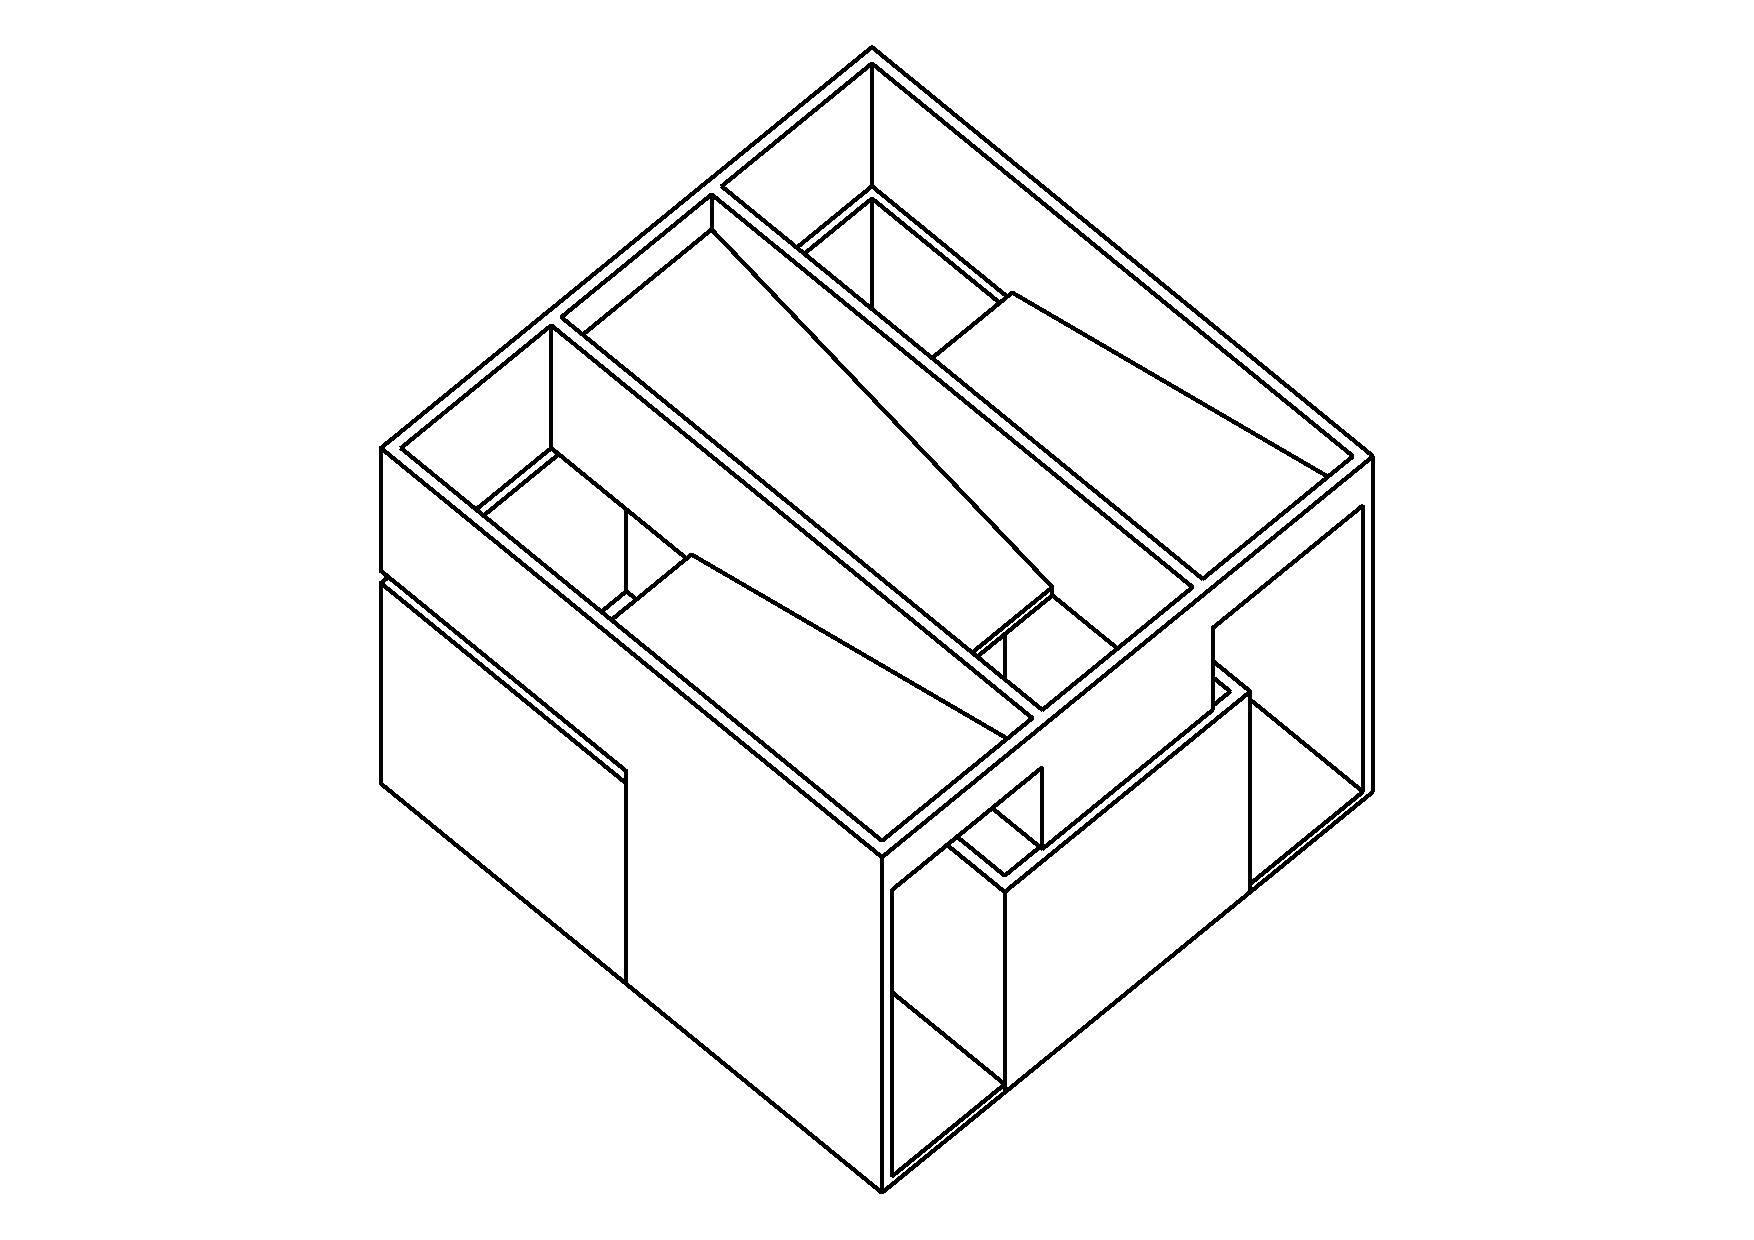
\includegraphics[width=\textwidth]{Graphics/Reservoir_final/DEUXIEME_BROUILLON.pdf}
    \caption{Deuxième brouillon}
    \label{fig:B2}
\end{figure}

\subsection{Troisième brouillon}
Vu que l'assemblage avec des vis de plus de 4 mm n'est pas possible pour certains éléments du deuxième brouillon (i.e. les cubes) et que la fabrication par fraisage à partir d'un seul bloc est bien trop coûteux et inefficace, nous avons remanié le brouillon en respectant ces aspects. La forme allongée des containers nous a permis de supprimer les rampes au-dessous du réservoir et donc de diminuer le nombre d'éléments.

\begin{figure}[h]
    \centering
    \includegraphics[width=0.7\textwidth]{Graphics/Reservoir_final/TROISIEME_BROUILLON.pdf}
    \caption{Troisième brouillon}
    %\label{fig:B3}
\end{figure}

%\section{Acheminement}
%Pour l'acheminement des billes, nous avons tout d'abord imaginé un réservoir au fond incliné contenant les billes, et débouchant sur une série de roues dentées qui permettent de réguler le flux de billes.

%Ensuite, nous avons dû imaginé un mécanisme permettant d'acheminer les billes vers la zone de tri de manière régulée, tout en évitant absolument le coincement. Ainsi, l'idée de routes dentées dimensionnées pour contenir exactement une bille dans chaque compartiment s'est imposée comme étant la meilleure. En effet, une série de roues dentées décalées d'une dent (...) permet de prélever un nombre précis de billes en vue du tri.
%Les routes dentées sont actionnées grâce à une manivelle qui transmet le mouvement de rotation grâce à un arbre.

%\section{Tri}
%Pour le tri des billes, nous avons développé un système de rails parallèles, s'écartant par pallier. Cela permet de récolter les petites billes d'abord, les moyennes ensuite et finalement les plus grosses. L'écartement par pallier permet aussi d'éviter le coincement. En effet, nous avions tout d'abord pensé à un écartement progressif des rails, mais les billes ralentissent alors fortement avant de tomber, ce qui peut provoquer l'arrêt des billes suivantes. En effet, plus le diamètre de la bille se rapproche de la distance entre les rails, plus la bille descend, et son axe de rotation se rapproche de son axe de symétrie horizontal. Il en résulte une augmentation de la vitesse de rotation de la bille, et une diminution de sa vitesse horizontale. Ainsi, la bille qui suit risque de frotter contre celle qui ralentit, et la force de frottement entre les deux, amplifiée par l'augmentation de la vitesse angulaire de la première bille, risque de stopper les billes sur le rails, bloquant alors le mécanisme.
\chapter{Justifications des choix}

\section{Réservoir pour les billes mixtes}

\subsection{Dimensionnement}
Les parois du réservoir initial mesurent 15 mm de hauteur: associées au fond en feutre, elles permettent d'éviter que des billes ne soient perdues si elles sont versées rapidement, tout en économisant de la matière par rapport à des parois sur-dimensionnées. 
Ensuite, la pente de \ang{3} du fond du réservoir assure la descente des billes vers le distributeur, mais avec une vitesse modérée. De plus, les interactions des billes entre elles renforcent ce phénomène de ralentissement.
Finalement, nous avons calculé la surface du réservoir comme suit:
\[S = L \cdot l = \SI{99}{\milli\metre} \cdot \SI{165}{\milli\metre} = \SI{16335}{\milli\metre\squared}\]
Où $L$ est la longueur du fond du réservoir, et $l$ la largeur.
Ainsi, dans le pire des cas, soit \num{300} billes de \SI{7}{\milli\metre} de diamètre, ces dernières peuvent se répartir sur l'ensemble du fond du réservoir sans se superposer, si elles sont versées avec soin. En effet, la surface de répartition est donnée par:
 Nous avons calculé le volume des réservoirs comme suit:
\[S\textsubscript{max} = (\SI{7}{\milli\metre})^{2} \cdot \num{300} \cdot d \approx {\num{7}}^{3} \cdot 300 \cdot 0.9 = \SI{13230}{\milli\metre\squared}\]
Où \(d = \frac{ \pi }{2\sqrt{3}} \approx \num{0.75}\) est la densité surfacique de l'arrangement compact de billes.
Cela permet déjà de réduire le risque de problèmes au niveau du distributeur, même si d'autres précautions ont été prises plus loin pour exclure tout coincement.

\subsection{Assemblage}
Pour assembler le fond du réservoir avec les parois, nous avons choisi d'utiliser des goupilles, car des vis aurait exigé un perçage chanfreiné des parois du réservoir pour fixer une vis à tête conique, mais l'épaisseur de 6 mm ne permet pas: cela aurait affaibli le montage. A l'opposé, les goupilles peuvent être fixées grâce à un simple perçage, ce qui renforce l'assemblage.

\section{Acheminement}
\subsection{Choix final}
Après l'évaluation de toutes les options notre choix fut le suivant:
\begin{itemize}
	\item \num{12} cylindres perforés de diamètre \SI{60}{\milli\metre} avec \num{10} trous arrondis de profondeur \SI{5.586}{\milli\metre} montés sur une barre
%à discuter
	\item une barre de diamètre \SI{8}{\milli\metre} avec un collet (diamètre \SI{6}{\milli\metre}) aux deux extrémités pour la fixer dans deux roulements à billes. À l'extrémité droite se trouve un taraudage (M4) pour fixer la pièce tenant la manivelle.
	\item une grande fixation quasi-symétrique des deux cotés. Elle contiennent un évidement pour serrer les roulements à billes, des extrusions avec des taraudages pour fixer le cache et deux extrusions pour fixer le réservoir mixte et les rails. La seule différence entre la fixation du côté gauche et celui du côté droite est qu'à droite au centre de l'évidement se trouve un alésage passant à travers pour pouvoir visser la fixation de la manivelle à la barre 
	\item une pièce pour tenir la manivelle qui consiste d'un cylindre avec un carré d'entraînement d'un côté et un filetage M4 de l'autre
	\item une manivelle
%à décider
	\item un couvercle empêchant que les billes tombent dans les derniers \ang{30} de la rotation.
\end{itemize}


\subsubsection{Vitesse de tri}
La surface de contact entre les cylindres perforés et le réservoir est de \SI{96}{\milli\metre}. Le diamètre moyen d'une bille est \SI{6}{\milli\metre}. Sur la surface de contact se trouveront alors

\[\frac{\num{96}}{\num{6}} = \num{16}\]
billes. À la surface de contact, il y a \num{8} trous à la fois à disposition qui seront donc tous remplis. Ainsi, lorsque la manivelle fait un tour entier, on pourra potentiellement acheminer 
\[(\text{nombre de trous par cylindre}) \cdot (\text{nombre de cylindres}) = \num{10} \cdot \num{12} = \num{120}\]
billes.
On considère que jusqu'à ce qu'il ne reste que \num{50} billes dans le réservoir, la surface de contact sera remplie entièrement (pour avoir encore plus de certitude calculera avec une marge de sécurité de \num{0.9}).
Alors si on commence dans une position de départ où les billes peuvent directement entrer et qu'on achemine \num{120} billes par tour on va
% SIUNITX fixed until here (Robin)
\[\frac{\theta}{\omega} = \frac{\frac{(250 \cdot 2)\pi}{120 \cdot 0.9}}{\frac{2\pi}{s}} = \frac{250}{108} \ s = 2.315 \ s \]
acheminer 250 billes en \SI{2.315}{\s} avec une vitesse de rotation d'un tour par seconde.
Les 50 dernières billes vont s'acheminer un peu plus lentement vu que la probabilité qu'ils tombent directement sur un trou diminue. Au lieu de faire un calcul exponentiel très compliqué on va partir de l'approximation qu'ils soient entraînes avec une certitude de \SI{50}{\percent}. Ce qui fait que
\[\frac{\theta}{\omega} = \frac{\frac{(50 \cdot 2)\pi}{120 \cdot 0.5}}{\frac{2 \pi}{s}} = \frac{50}{60} \ s = 0.833 \ s\]
0.833 secondes supplémentaires suffiront.
En un total de 3.148~s toutes les billes auront alors passé le mécanisme d'acheminement.
%tilda correct?
\subsection{Acheminement}
La première question qui se pose, c'est si les billes de diamètre 5 vont rester dans leurs cases pendant les premiers \ang{150} de leur tour (cf. figure en dessous). Car si la condition centripète n'est pas remplie constamment, la force centrifugale (dans le repère tournant) dirigerait les petits billes vers les arêtes des dents. Vu que les plus petites billes ont un radius (2.5) égal à la distance entre l'arête et le couvercle ceci pose un risque de coincement. Si nous considérons la figure ci-dessous, l'accélération centripète est donnée par:
% figure manque
\[ma_{c} = mg \cdot \sin\theta\]
Pour une vitesse de rotation de \(\frac{2 \pi}{s}\) la condition centripète reste remplie pour tout angle supérieur à %\ang{?}
\[\cancel{m} \cdot g \ sin\theta = \cancel{m} \frac{v^{2}}{R + r} = \cancel{m} \cdot \omega^{2} \ (R +r)\]
\[sin \theta = \frac{\omega^{2} \ (R + r)}{g} = \frac{\frac{2 \pi}{s^{2}}\ (24.414mm + 2.5mm)}{10\frac{m}{s^{2}}} = \frac{\frac{4 \pi^{2}{s^{2}}} \ (26.914mm)}{10\frac{m}{s^{2}}} = \]
%letzte gleichung ausrechnen
Il reste à vérifier deux choses. Est-ce que le centre de masse de la bille restera dans la zone verte (voir figure en dessous) entre $\theta$ = voir en haut et $\theta$ = 0.
%figure manque
\subsubsection{Partie Pink 2}
Vu que dans cette partie de la rotation la condition centripète n'est plus satisfaite, la bille va commencer à rouler hors de son logement. Pour faciliter les calculs on va considérer que la bille soit un point de masse qui se déplace sans friction en direction du couvercle pendant $\theta = $%voir en haut
et $\theta = 0$. 
Cette approximation assez forte est tout à fait valable. Car si je calcule l'accélération de la bille sans prendre la friction, la résistance au roulement et l'énergie convertie en énergie de rotation en compte je majore celle-ci. C'est-à-dire que si la bille ne sort pas de la zone verte dans le calcul aproximé, elle ne le ferait sûrement pas en réalité.\\
On a alors l'équation pour la deuxième loi de Newton suivante (dans le repère tournant):
\[ma = m \frac{\omega^{2}}{(R + r)}\]
\[a = \omega \ (R + r) = \frac{4 \pi^{2}}{s^{2}} \ (26.914mm) = \]
%à calculer et si nécessaire inclure friction
Le déplacement $\Delta\theta$ entre $\theta =$ voir en haut et $\theta = 0$ va prendre
\[2 \pi \estimates 1 s\]
\[\therefore t = \frac{x \ s}{2 \pi} = \]
%calcul manque
et donc la bille se déplacera de (?) 
\[s = \frac{1}{2} \ a \ t^{2} = ? \]
.
Ceci est inférieur à la distance 
\[d = b - 2r = 8.086mm - 2 \times 2.5mm = 3.086mm\]
où b est la distance entre le fond et le couvercle et on en soustrait 2r cas le centre de masse se trouve à distance r du fond et la bille n'a justement pas le droit de se trouver qu'à distance r du couvercle).

\subsubsection{Partie Pink 3}
La deuxième chose à vérifier est, si la bille maintenant en chute, tombera plus lentement que son logement et ainsi bloquera le mécanisme (si elle tombe plus vite ceci n'est pas problématique - vu que le mécanisme tourne dans la direction de sa chute ça se débloquerait soi-même). Ceci ne serait pas du tout problématique si la bille se trouvait en chute libre car
\[v_{1} = v_{0} + a \ t > v_{0} , \Leftrightarrow a,t > 0\]
Mais vu que dans cette partie la bille roulera le long du couvercle une partie de l'énergie potentielle sera transformée en énergie de rotation.
À $\theta = 0$ on a:
%image manque
\[E_{0} = m\ g\ h + \frac{1}{2}\ m\ {v_{0}}^{2} \ \text{où} \ v_{0} = \omega_{cylindre}\ (R + r) = \frac{2\pi}{s}\ 26.914mm = 0.017 \frac{m}{s}\]
À $\theta = \ang{-45}$ on a:
\[E_{1} = \frac{1}{2}\ m\ v_{1}^{2} + \frac{1}{2}\ I\omega_{bille}\]
\begin{equation}
E_{0} = E_{1}
\end{equation}
\begin{equation}
m\ g\ h + \frac{1}{2}\ m\ (\omega_{cylindre}\ (R + r))^{2} = \frac{1}{2}\ m\ v_{1}^{2} + \frac{1}{2}\ I\omega_{bille}
\end{equation}
\begin{equation}
\cancel{m}\ g\ h + \frac{1}{2}\cancel{m}\ (\omega_{cylindre}\ (R + r))^{2} = \frac{1}{2}\cancel{m}\ v_{1}^{2} + \frac{1}{\cancel{2}}\ \frac{\cancel{2}}{5}\cancel{m}\ r^{2}\omega_{bille}
\end{equation}
\begin{equation}
\cancel{m}\ g\ h + \frac{1}{2}\cancel{m}\ (\omega_{cylindre}\ (R + r))^{2} = \frac{1}{2}\cancel{m}\ v_{1}^{2} + \frac{1}{\cancel{2}}\ \frac{\cancel{2}}{5}\cancel{m}\ r^{2}\omega_{bille}
\end{equation}
\begin{equation}
\omega_{bille} = \frac{v_{1}}{r}
\end{equation}
\begin{equation}
g\ h + \frac{1}{2}\ (\omega_{cylindre}\ (R + r))^{2} = \frac{1}{2}\ v_{1}^{2} + \frac{1}{5}\ r^{2}\frac{v_{1}}{r}
\end{equation}
Par contre, ce calcul montre que $v_{1}$ sera supérieur à $v_{0}$ malgré l'énergie perdue en rotation. Ainsi, la preuve est fournie qu'il y aura pas de blocage pendant l'acheminement des billes. Dans le pire des cas où une "erschütterung" (?) ou un incident semblableme imprévisible aura comme conséquence qu'une bille se coince, le couvercle pourrait toujours s'enlever à l'aide d'un tournevis (?).
\subsection{Consommation d'énergie et sollicitation}
Une autre condition nécessaire au fonctionnement de notre mécanisme est s'il se laisse opérer avec un effort acceptable. L'acheminement fut conçu afin de minimiser les surfaces de contact avec les éléments statiques afin de minimiser la friction. En considérant le dessin ci-dessous on s'aperçoit que tout les moments de force en jeu se résument dans l'équation suivante:
%dessin manque
%formule manque
où alfa (?) %formule 
et où on considère le pire des cas ou on a toute les q * 12 cases remplis d'une bille avec diamètre 7 (donc contact avec le couvercle (?) et le fond de la dent (?) et ainsi deux fois une résistance au roulement).
En résolvant ceci selon $F_{main}$ on obtient
%formule fmain =
Le travail fourni pas l'utilisateur est alors 
% fmain * 2 pi
.
L'énergie investi par cycle suit ainsi du calcul
%formule
\subsection{Débloquage}
Finalement il reste à évaluer s'il y a un empilement possible dans les "trous". Un tel empilement aurait comme conséquence que les billes soient très proche sur les rails et se freinent les uns  les autres où même que sa bloque l'acheminement.
\subsubsection{Calculs}
L'idée initiale fut de mettre le couvercle à une distance de 2.5 mm des cylindres perforés pour que s'il y a un empilement de deux billes de 5mm (ce qui représente le seul cas problématique) la bille de dessus soit heurté contre son centre de masse et ainsi repulsé.
Mais considérons le dessin ci-dessous (à 35 degrés (?) de l'horizontale, c'est-à-dire 5 degrés (?) de rotation après que la bille soit soulevée)
%Dessin manque
Si on impose l'équilibre sur la bille extérieur
%formules
on s'aperçoit que \textit{a} devrait être inférieur à (?) pour que la bille reste en position. Par contre en pratique \textit{a} vaut (?) ce qui signifie que les billes ne s'empileront pas. Et vu que l'acheminement se fait en 3.148 secondes tout empilement devant à la surface de contact sera négligeable. (?)

\section{Séparation et rails}

\section{Réservoir pour les billes triées}
La version finale du réservoir pour les billes triées était le troisième brouillon. Au contraire du premier brouillon, la version finale nous permet d'enlever les containers avec les billes triées séparément, et cela sans que la construction des pièces soit difficile, ce qui a exclu le deuxième brouillon. Voici ces deux raisons principales en plus de détail:

\subsection{Containers flexibles}
Quelle que soit l'utilisation des billes triées, la flexibilité des containers, qui permettent d'enlever toutes les billes triées de la même taille en même temps, est bien utile lors de l'utilisation future de la machine. Son efficacité en service est donc bien meilleure que si l'on devait enlever toutes les billes à la main d'un container fixe. Le positionnement exact des containers est garanti par une plaque %{insérer lien dessin sol}
qui entoure les pieds de chacun des containers. Le jeu pour enlever les containers est d'un millimètre en haut ainsi qu'en bas. C'est assez grand pour qu'ils ne se coincent pas, et assez petit pour que la distance entre le haut du container et la prochaine pièce soit de 4 mm, ce qui garantit que même les billes les plus petites trouvent leur chemin dans le bon réservoir, une fois tombées à travers les rails.

\subsection{Usinage}
Nous avons décidé d'augmenter le nombre de pièces afin de simplifier leur usinage. Parmi les pièces utilisées, il n'y a aucune pièce qui ne pouvait pas être usiné par des processus courants, certaines même sans assistance par ordinateur. La décomposition en pièces faciles à usiner est un avantage pour la production, mais pas pour l'assemblage de la machine. Si l'on voulait lancer la machine en production en grande série, il faudrait reconsidérer ce choix. En grand nombre, même des pièces plus complexes sont moins chères car les coûts de la configuration de l'usinage peuvent être répartis sur plusieurs pièces et forment donc une plus petite partie du prix de la pièce. Nous avons estimé que pour notre projet, le surcroît des dépenses se compense facilement par l'économie réalisée pendant l'usinage.

En outre, nous avons fait intervenir des parois qu'il est possible d'acheter bon-marché. En découpant une paroi, nous obtenons une pièce qui s'utilise facilement comme partie d'un container. Comme déjà évoqué, nous avons rejeté l'idée d'ajuster la taille de chaque réservoir à la taille des billes correspondantes, pour augmenter la simplicité dans la production. 

\subsection{Dimensionnement}
Le dimensionnement des cubes se déroulait en prise en compte de la taille des billes. Dans le pire des cas, les 300 billes sont de la même taille : les réservoirs doivent alors être capables de contenir 300 billes de la taille respective. Pour simplifier la construction, les cubes ont tous la même taille sans respecter la taille des billes.
Nous avons calculé le volume des réservoirs comme suit:
\begin{equation}
    V = 7^3\ 300\ d \approx 7^3\ 300\ 0.75 = 77'175\ mm^3
    \label{eq:volumereservoirfin}
\end{equation}

Où \(d = \frac{ \pi }{3\sqrt{2}} \approx 0.75\) est la densité volumique de l'empilement compact de billes.
La taille du rayon interne de la paroi se calcule comme suit:

\begin{equation}r\textsubscript{int}\geq\sqrt{\frac{2\ V}{\pi\ l}}=\sqrt{\frac{2\ 77'175\ mm^3}{\pi\ 90\ mm}} \approx 23.4\ mm \label{eq:rayonreservoirfin}\end{equation}

Avec \(V=77'175\ mm^3\) calculé par la formule \ref{eq:volumereservoirfin} et \(l=90\ mm\) la longueur interne adaptée à la largeur des rails. En ajoutant un petit facteur de sécurité si les billes ne s'empilent pas de la manière la plus compacte possible, et en fixant l'épaisseur de la paroi de \(2\ mm \), nous avons obtenu un rayon externe de la paroi de \(r\textsubscript{ext}=27\ mm\). Pour que les billes ne fassent pas trop de bruit lors du choc au réservoir, nous avons prévu un revêtement en feutre d'une épaisseur d'un millimètre. Le rayon interne mesure alors \(24\ mm \), ce qui respecte toujours la limite qu'on a calculé par la formule \ref{eq:rayonreservoirfin}.

\include{Sections/Descriptifs}
\chapter{Dessin d'ensemble}

\includepdf{Documents/Dessin_ensemble/ENSEMBLE1_Calque.pdf}
\includepdf[pages=1,fitpaper]{Documents/Dessin_ensemble/ENSEMBLE2_Calque.pdf}
\includepdf[pages=1,fitpaper]{Documents/Dessin_ensemble/ENSEMBLE3_Calque.pdf}
\chapter{Dessins de détail - pièces usinées}
\chapter{Dessins de détail - pièces achetées}
\chapter{Plan \& notice de montage}
Le montage de la machine se fait grâce aux 7 étapes suivantes:

\begin{enumerate}
    \item Montage des réservoirs finaux
    \item Montage des cylindres perforés sur l'axe du distributeur
    \item Montage des goupilles et des roulements dans les parois gauches et droites
    \item Montage du distributeur et du couvercle sur la paroi gauche
    \item Montage des composantes centrales
    \item Montage de la paroi droite et la manivelle
    \item Montage des plaques du fond
\end{enumerate}

\newpage

\begin{enumerate}

\begin{figure}
    \centering
    \includegraphics[width=0.6\textwidth]{Graphics/Montage/1.pdf}
    \caption{Montage 1}
    \label{fig:Montage1}
\end{figure}

\item A l'aide d'une clé allen de 3, assembler deux bords réservoir pour billes triées (pièces \No6), un tube réservoir pour billes triées (pièce \No7), deux pieds réservoir pour billes triées (pièce \No5), avec deux vis M4x10 (pièce \No21).

\newpage

\begin{figure}
    \centering
    \includegraphics[width=\textwidth]{Graphics/Montage/2.pdf}
    \caption{Montage 2}
    \label{fig:Montage2}
\end{figure}

\item  Chauffer les cylindres perforés (pièce \No14) jusqu'à une température de \SI{275}{\degreeCelsius}, avant de les chasser sur l'axe du distributeur (pièce \No13). Les cylindres sont ainsi assemblés par serrage sur l'axe.

\newpage

\begin{figure}
    \centering
    \begin{subfigure}[h]{0.45\linewidth}
        \includegraphics[width=\linewidth]{Graphics/Montage/3A.pdf}
    \end{subfigure}
    \hfill
    \begin{subfigure}[h]{0.45\linewidth}
        \includegraphics[width=\linewidth]{Graphics/Montage/3B.pdf}
    \end{subfigure}
    \caption{Montage 3}
    \label{fig:Montage3}
\end{figure}

\item Chasser les goupilles (pièce \No18) dans leurs logements sur les pièces fixation gauche (pièce \No4) et fixation droite (pièce \No3). Chasser les roulements à bille (pièce \No17) dans les trous de diamètre \SI{7}{\mm} des deux pièces fixation.

\newpage

\begin{figure}
    \centering
    \includegraphics[width=\textwidth]{Graphics/Montage/4.pdf}
    \caption{Montage 4}
    \label{fig:Montage4}
\end{figure}

\item Monter l'axe et les cylindres ainsi que le cache (pièce \No15) sur la pièce fixation gauche.

\newpage

\begin{figure}
    \centering
    \includegraphics[width=\textwidth]{Graphics/Montage/5.pdf}
    \caption{Montage 5}
    \label{fig:Montage5}
\end{figure}

\item Chasser le fond réservoir pour billes mixtes (pièce \No12) sur la pièce fixation gauche, grâce aux goupilles. Assembler, à l'aide d'une clé allen de 2.5, le bord avant et le bord arrière (pièces \No11) avec la pièce fixation gauche, grâce à deux vis M4x12 (pièces \No19). Assembler ensuite les deux limitations épaisses (pièce \No8) et fines (pièce \No9) dans la pièce fixation gauche. Chasser finalement le séparateur (pièce \No10) sur les deux goupilles.

\newpage

\begin{figure}
    \centering
    \includegraphics[width=\textwidth]{Graphics/Montage/6.pdf}
    \caption{Montage 6}
    \label{fig:Montage6}
\end{figure}

\item A l'aide d'une clé allen de 2.5, assembler la pièce fixation droite sur l'ensemble construit jusqu'à présent, grâce à deux vis M4x12 (pièces \No19). Visser ensuite la manivelle (pièce \No16) sur le filetage de l'axe. 

\newpage

\begin{figure}
    \centering
    \includegraphics[width=0.5\textwidth]{Graphics/Montage/7.pdf}
    \caption{Montage 7}
    \label{fig:Montage7}
\end{figure}

\item Finalement, assembler la plaque de fond (pièce \No1) et la pièce fixation des réservoirs (pièce \No2) grâce à 6 vis M4x16 (pièces \No20).

\end{enumerate}
\chapter{Mode d'emploi}
Le fonctionnement de la machine est assuré par une seule personne, grâce à la manivelle. Avant de commencer le tri, l'utilisateur doit verser avec précaution les 300 billes dans le réservoir pour billes mixtes, situé sur le dessus de la machine. Il peut alors les répartir avec la main sur le fond du réservoir, s'il constate un empilement important avant le distributeur.

Pour débuter le tri des billes, l'utilisateur tourne avec sa main droite la manivelle dans le sens des aiguilles d'une montre. Il peut poser sa main gauche sur le réservoir mixte sans danger, ce qui stabilise d'avantage la machine. Il ne faut cependant pas mettre les doigts dans la partie découverte du distributeur lorsque l'on tourne la manivelle, pour des raisons de sécurité. La vitesse de rotation de la manivelle doit être d'environ un tour par seconde, pour assurer un tri optimal des billes. Le temps nécessaire pour trier 300 billes est inférieur à 5 secondes.

A la fin du processus, l'utilisateur peut récupérer les billes séparées en fonction de leur taille dans trois réservoirs distincts situés dans le fond de la machine. Depuis le côté du distributeur, le premier réservoir contient les billes de 5 mm, le deuxième celles de 6 mm, et le dernier les billes de 7 mm. Ces réservoirs peuvent facilement être sortis et remis dans leur emplacement.
%version alternative:
%Le fonctionnement de la machine est assuré par une seule personne, grâce à la manivelle. L'utilisation se fait comme suit:
%\begin{itemize}
%    \item Versez avec précaution les 300 billes dans le réservoir pour billes mixtes, situé sur le dessus de la machine. En cas d'empilement important veuillez les répartir avec la main sur le fond du réservoir.
%    \item Tournez avec votre main droite la manivelle dans le sens des aiguilles d'une montre à une vitesse d'un tour par seconde. (Ça ne pose aucun danger de poser votre autre main sur la machine, au contraire ceci la stabilisera.)
%    \item Récupérez les billes triés en sortant le réservoir correspondant (Depuis le côté de la manivelle, le premier réservoir contient les billes de 5 mm, le deuxième celles de 6 mm, et le dernier les billes de 7 mm.
%\end{itemize}
\chapter{Annexe}

\section{Pièces achetées}
\subsection{Liste des pièces}
\begin{table}[htbp]
    \centering
    \begin{tabular}{|c|c|c|c|}
        \hline
         & Fournisseur & \No de référence \\
        \hline
        Manivelle & MISUMI & \texttt{DA80RG} \\
        \hline
        Roulement & Engrenages HPC & \texttt{S686ZZ} \\
        \hline
        Goupille & - & ISO 8752-4$\times$10-Ac\\
        \hline
        Vis & - & ISO 10642-M4$\times$12-8.8 \\
        \hline
        Vis & - & ISO 4762-M4$\times$10-8.8 \\
        \hline
    \end{tabular}
    \caption{Liste des pièces achetées avec fournisseur}
    %\label{tab:listepiècesachetées}
\end{table}


\subsection{Spécification du fournisseur}
Sur les pages suivantes se trouvent les fiches techniques de la manivelle et des roulements.

\includepdf{Documents/Pieces_achetees/nda_da-e.pdf}
\includepdf{Documents/Pieces_achetees/S_ZZ_1.pdf}
\includepdf{Documents/Pieces_achetees/S_ZZ_2.pdf}

\end{document}